
\newcommand{\numTD}{TD3}
\newcommand{\themeTD}{Codages Informatiques}

\begin{center}
\begin{tabular}{|p{2cm}c|}
\hline
{
\includegraphics[width=1.8cm,viewport=0 0 337 248]{../images/sorbonne.png}} & \raisebox{2ex}{\begin{Large}\textbf{M1SOL020}\end{Large}}\\
2019-2020& \raisebox{2ex}{\begin{Large}\textbf{ Epistémologie de l'Informatique}\end{Large}}\\
&  \begin{large}\textbf{\numTD}\end{large} \\
&  \begin{large} \textbf{\themeTD}\end{large} \\
& Gaël Lejeune, Sorbonne Université \\
& \tiny{Inspiré d'Agnès Delaborde 2015-2016}\\
\hline
\end{tabular}
\end{center}


\hrule
%%%%%%%%%%%%%%%%%%%%%%%%%EN-TETE%%%%%%%%%%%%%%%%%%%%%%%%%%%%%
%\renewcommand{\contentsname}{Sommaire du TD}
%\tableofcontents

\noindent\fcolorbox{red}{lightgray}{
\begin{minipage}{12cm}
\section*{Objectifs}

\begin{itemize}
 \item Comprendre les codages binaires, décimaux, et hexadécimaux
 \item Appréhender le codage des caractères (ASCII et ASCII étendu)
\end{itemize}
\end{minipage}
}



\section{Codage décimal (base 10)}
\begin{itemize}
 \item  Que signifie " base 10 " ?
 \item  La numération romaine est-elle en base 10 ?
\end{itemize}

\section{Codage binaire (base 2)}

 Ici chaque élément peut coder 2 valeurs (0 ou 1) là où le système décimal encode 10 valeurs différentes dans chaque élément (0 à 9). Pour la justification de l'utilisation du binaire, allez voir la partie \textit{Why Binary?} dans la partie Aprrofondissement en fin de TD.

\begin{itemize}
 \item  Que signifie numération binaire positionnelle ?
\end{itemize}
\subsection{Du binaire au décimal}

\begin{itemize}
 \item  Partez de cette définition pour compléter le tableau ci-dessou et convertir en base décimale les nombres exprimés en base 2 : %. Indiquez leur valeur en base décimale :
\end{itemize}

\begin{tabular}{p{2cm}|p{10cm}|p{2cm}}
Binaire		&Analyse	&Décimal\\
\hline
0		&		&	\\
\hline
101		&$1*2^2 + 0*2^1 + 1*2^0$		&5	\\
\hline
1		&		&	\\
\hline
110010		&		&	\\
\hline
111101		&		&	\\
\end{tabular}


\subsection{Du décimal au binaire}
\begin{itemize}
 \item En utilisant la méthodologie proposée ci-dessous, convertissez en binaire la série de nombres en base 10 qui suit :%xprimez ces nombres en base binaire : 
\end{itemize}

\textbf{Méthodologie :}

%\begin{table}

\begin{tabular}{l|l|l|l|l|l|l|l|l|l}
Binaire		&   0	&    0	&    0	&    0	&    0	&    \textbf{1}	&    0	&    0	&    \textbf{1}	\\
\hline
Décomposition	&$1*2^9$ & $1*2^8 $ &$1*2^7$ & $1*2^6$ & $1*2^5$ & \textbf{$1*2^4$} & $1*2^3$ & $1*2^1$ & $1*2^0$\\
\hline
Valeur décimale	&256	&128	&64	&32	&16	&\textbf{8}	&4	&2	&\textbf{1}\\	
%\hline
%Valeurs utilisées	&0	&0	&0	&0	&0	&\textbf{8}	&0	&0	&\textbf{1}\\
\end{tabular}
\vspace{0.2cm}


\textit{Lecture : Si je veux représenter 9 je dois trouver la somme correspondante dans la ligne des valeurs décimales. En l'occurrence, c'est 8 + 1. Je peux donc remonter à la ligne Binaire pour récupérer les "1" dont j'ai besoin, le reste ce sont des "0 : $8_{\text{10}}$ = $000001001_{\text{12}}$ }
%Je vois dans la ligne des "chiffres en binaire" que j'obtiens 000001000. Je peux retirer les premiers zéros qui ne sont pas nécessaires dans cet exercice, et dire donc que 8(10) = 1000(2).

%\end{table}

\textbf{Tableau à compléter :}

%\begin{tabular}{l|l|l}
\begin{tabular}{p{2cm}|p{10cm}|p{2cm}}
Décimal		&Analyse	&Binaire\\
\hline
0		&		&	\\
\hline
1		&		&	\\
\hline
2		&		&	\\
\hline
3		&		&	\\
\hline
4		&		&	\\
\hline
5		&		&	\\
\hline
6		&		&	\\
\hline
7		&		&	\\
\hline
8		&		&	\\
\hline
9		&$9=8+1 = 1*2^3 + 0*2^2 + 0*2^1 + 1*2^0$		&1001	\\
\hline
32		&		&	\\
\hline
66		&		&	\\
\hline
128		&		&	\\
\hline
255		&		&	\\
\end{tabular}


 \begin{itemize}
   \item  Quel est l'entier maximal que l'on puisse coder sur 16 bits ?
 \end{itemize}

\section{Addition en Binaire}

\subsection{Additions en binaire}

% \begin{itemize}
%   \item  Additionnez ces nombres à la main en suivant les règles d’addition proposées dans le tableau ci-dessous :
% \end{itemize}

Règles d'additions en binaire:
\begin{itemize}
  \item$0 + 0 = 0$, on pose 0
  \item$0 + 1 = 1$, on pose 1
  \item$1 + 1 = 10$ : on pose 0 et on retient 1
  \item$1 + 1 + \text{retenue} =11$ : on pose 1 et on retient 1
\end{itemize}

Explication pour \textbf{$1010_{(2)} + 0011_{(2)}$} (on lit de droite à gauche):

\vspace{0.2cm}

\begin{tabular}{l|p{2.5cm}|p{3cm}|p{3cm}|p{2.5cm}}
	&	1	&0	&1	&0\\
\hline
+	&	0	&0	&1	&1\\
\hline
\hline
Opérations	&	on pose \textcolor{blue}{\textbf{1}}&0 + la \textcolor{red}{\textbf{retenue}}, on pose \textcolor{blue}{\textbf{1}} &on pose \textcolor{blue}{\textbf{0}} et on \textcolor{red}{\textbf{retient}} 1&on pose \textcolor{blue}{\textbf{1}}\\
\hline
Résultat	&1	&1	&0	&1	\\
\end{tabular}

\vspace{0.2cm}
On a bien le résultat correspondant en système décimal : $10_{(10)} + 3_{(10)} = 13_{(10)}$

\begin{itemize}
  \item A vous pour : $1111_{(2)} + 1111_{(2)}$
\end{itemize}



\subsection{Conversion et addition}

 \begin{itemize}
   \item  Convertissez ces nombres en binaire, et additionnez les : $19_{\text{(10)}}$ + $71_{\text{(10)}}$
 \end{itemize}

\section{Codage hexadécimal (base 16)}
 \begin{itemize}
 \item  Quels sont les 16 chiffres du système hexadécimal ?
 \item  Convertissez $4D5_{(16)}$, et $F48A_{(16)}$ en décimal.
 \item  Addition en hexadécimal. En vous appuyant sur le tableau \ref{table_hexa}, combien vaut D + C en base 16 ? Exprimez ensuite ce calcul en base 10.
 \end{itemize}

\begin{table}
\caption{Table d'addition hexadécimale\label{table_hexa}}
\begin{tabular}{>{\columncolor{lightgray}}c|c|c|c|c|c|c|c|c|c|c|c|c|c|c|c|c}
\rowcolor{lightgray}+	&0	&1	&2	&3	&4	&5	&6	&7	&8	&9	&A	&B	&C	&D	&E	&F\\
\hline
0	&0	&1	&2	&3	&4	&5	&6	&7	&8	&9	&A	&B	&C	&D	&E	&F\\
\hline
1	&1	&2	&3	&4	&5	&6	&7	&8	&9	&A	&B	&C	&D	&E	&F	&10\\
\hline
2	&2	&3	&4	&5	&6	&7	&8	&9	&A	&B	&C	&D	&E	&F	&10	&11\\
\hline
3	&3	&4	&5	&6	&7	&8	&9	&A	&B	&C	&D	&E	&F	&10	&11	&12\\
\hline
4	&4	&5	&6	&7	&8	&9	&A	&B	&C	&D	&E	&F	&10	&11	&12	&13\\
\hline
5	&5	&6	&7	&8	&9	&A	&B	&C	&D	&E	&F	&10	&11	&12	&13	&14\\
\hline
6	&6	&7	&8	&9	&A	&B	&C	&D	&E	&F	&10	&11	&12	&13	&14	&15\\
\hline
7	&7	&8	&9	&A	&B	&C	&D	&E	&F	&10	&11	&12	&13	&14	&15	&16\\
\hline
8	&8	&9	&A	&B	&C	&D	&E	&F	&10	&11	&12	&13	&14	&15	&16	&17\\
\hline
9	&9	&A	&B	&C	&D	&E	&F	&10	&11	&12	&13	&14	&15	&16	&17	&18\\
\hline
A	&A	&B	&C	&D	&E	&F	&10	&11	&12	&13	&14	&15	&16	&17	&18	&19\\
\hline
B	&B	&C	&D	&E	&F	&10	&11	&12	&13	&14	&15	&16	&17	&18	&19	&1A\\
\hline
C	&C	&D	&E	&F	&10	&11	&12	&13	&14	&15	&16	&17	&18	&19	&1A	&1B\\
\hline
D	&D	&E	&F	&10	&11	&12	&13	&14	&15	&16	&17	&18	&19	&1A	&1B	&1C\\
\hline
E	&E	&F	&10	&11	&12	&13	&14	&15	&16	&17	&18	&19	&1A	&1B	&1C	&1D\\
\hline
F	&F	&10	&11	&12	&13	&14	&15	&16	&17	&18	&19	&1A	&1B	&1C	&1D	&1E\\
\end{tabular}
\end{table}


\section{Codage des caractères (Codage ASCII)}

\begin{figure}
\caption{Table ASCII (source : \url{http://www.asciitable.com/})\label{tab:ascii}}
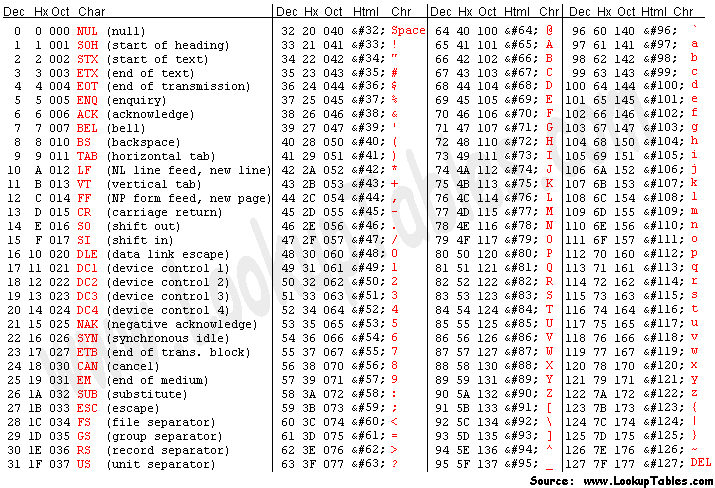
\includegraphics[width=1\textwidth]{../images/asciifull.png}
\end{figure}

 \begin{itemize}
 \item  Combien de codes différents existe-t-il dans l'ASCII standard (cf. Tableau \ref{tab:ascii} page \pageref{tab:ascii}?
 \item  Ce qui signifie qu'ils sont codés sur combien de bits ?
 \item  Observez la table ci-après. Quel problème peut survenir lorsqu'on écrit en français?
 \item  Quelle solution a été adoptée par l'ISO pour résoudre ce problème ? Quelle conséquence ?
 \end{itemize}

\noindent\fcolorbox{red}{lightgray}{
\begin{minipage}{15cm}
\subsection*{Approfondissement}
\begin{itemize}
  \item Pourquoi choisir le binaire pour les ordinateurs (\textit{Why Binary ?}) ? \url{https://www.youtube.com/watch?v=thrx3SBEpL8}
  \item Un convertisseur Binaire--Décimal--Hexadecimal :

 \url{http://sebastienguillon.com/test/javascript/convertisseur.html}


  \item Un exemple de problème d'encodage (ou \textit{encoding}) :
\end{itemize}

%\begin{figure}
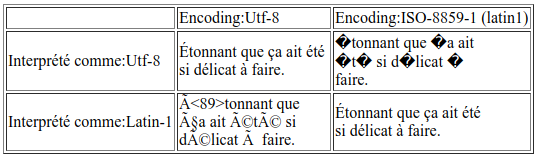
\includegraphics[width=.9\textwidth]{../images/TD3_encoding.png}
%\end{figure}

\end{minipage}
}
